\documentclass[10pt]{article}
\usepackage[polish]{babel}
\usepackage[utf8]{inputenc}
\usepackage[T1]{fontenc}
\usepackage{graphicx}
\usepackage[export]{adjustbox}
\graphicspath{ {./images/} }
\usepackage{amsmath}
\usepackage{amsfonts}
\usepackage{amssymb}
\usepackage[version=4]{mhchem}
\usepackage{stmaryrd}

\begin{document}
\begin{center}
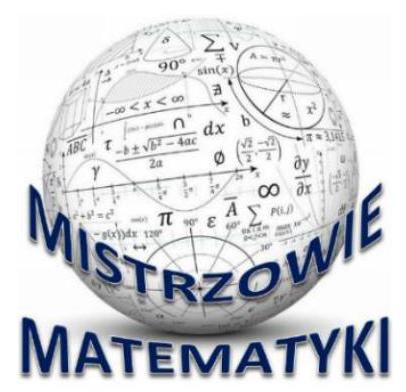
\includegraphics[max width=\textwidth]{2024_11_21_b8f206055f1c7e84536bg-1}
\end{center}

\begin{enumerate}
  \item Rozstrzygnij, czy szachownicę \(10 \times 10\) można pokryć 25-cioma klockami \(4 \times 1\).
  \item Zbadaj, czy szachownicę \(8 \times 8\) można obejść konikiem szachowym odwiedzając każde pole dokładnie jeden raz i startując w lewym dolnym rogu a kończąc w prawym górnym.
  \item \(\mathrm{Z} n^{2}\) płytek w kształcie trójkąta równobocznego o boku 1 ułożono trójkąt równoboczny o boku \(n\). Każda płytka jest z jednej strony biała, a z drugiej czarna. Ruch polega na wykonaniu następujących czynności: wybieramy płytkę P mającą wspólne boki z co najmniej dwiema płytkami, których widoczne strony mają kolor inny niż widoczna strona płytki P. Następnie odwracamy płytkę P na drugą stronę. Dla każdego \(n \geq 2\) rozstrzygnij, czy istnieje początkowe ułożenie płytek, pozwalające wykonać nieskończony ciąg ruchów.
\end{enumerate}

\end{document}